\documentclass[beamer, crop, multi = true, tikz]{standalone}

\usepackage{booktabs}
\usepackage{pgfplots}

\pgfplotsset{compat=newest}
\usepgfplotslibrary{groupplots}
\usepgfplotslibrary{polar}
\usepgfplotslibrary{smithchart}
\usepgfplotslibrary{statistics}
\usepgfplotslibrary{dateplot}
\usepgfplotslibrary{ternary}
\usetikzlibrary{arrows.meta}
\usetikzlibrary{backgrounds}
\usepgfplotslibrary{patchplots}
\usepgfplotslibrary{fillbetween}

\begin{document}
\begin{standaloneframe}[fragile]
\begin{tikzpicture}

\begin{scope}[xshift=-12cm, yshift=7.5cm]
	\tikzset{node distance=1.5cm, minimum size=1ex}
	\tikzset{class1/.style={circle, draw=black, fill=red!50}}
	\tikzset{class0/.style={circle, draw=black, fill=white}}

	\node[class1] (A1) {};
	\node[class1, right of=A1] (A2) {};
	\node[class0, below of=A1] (B1) {};
	\node[class0, right of=A2] (B2) {};
	\node[class0, below of=A2] (C1) {};
	\node[class0, below of=B2] (C2) {};
	\draw [-] (A1) -- (A2);
	\draw [-] (A1) -- (B1);
	\draw [-] (B1) -- (C1);
	\draw [-] (C1) -- (B2);
	\draw [-] (B2) -- (C2);
	\draw [-] (A2) -- (B2);
\end{scope}

\begin{scope}[xshift=-8.6cm, yshift=6.7cm]
	\draw[->, thick, shorten >=1ex, shorten <=1ex] (0,0.9) -- +(5,2.4) node [pos=0.5, above, sloped] {GNN with \( \lambda_1 \)} node [font=\LARGE, pos=1, xshift=1.3cm] {\( \rho \)=0.65};
	\only<1>{%
		\draw[->, thick, shorten >=1ex, shorten <=1ex] (0,0.3) -- +(5,0.8) node [pos=0.5, above, sloped] {GNN with \( \lambda_2 \)}  node [font=\LARGE, pos=1, xshift=1.3cm] {\( \rho \)=0.7};
	}
	\only<2>{%
		\draw[->, thick, shorten >=1ex, shorten <=1ex] (0,0.3) -- +(5,0.8) node [pos=0.5, above, sloped] {GNN with \( \lambda_2 \)}  node [font=\LARGE, pos=1, xshift=1.3cm] {\alert{\( \rho \)=0.7}};
	}
	\uncover<3->{%
		\draw[->, thick, shorten >=1ex, shorten <=1ex] (0,0.3) -- +(5,0.8) node [pos=0.5, above, sloped] {GNN with \alert{\( \lambda_2 \)}}  node [font=\LARGE, pos=1, xshift=1.3cm] {\alert{\( \rho \)=0.7}};
	}
	\draw[->, thick, shorten >=1ex, shorten <=1ex] (0,-0.3) -- +(5,-0.8) node [pos=0.5, above, sloped] {GNN with \( \lambda_3 \)}  node [font=\LARGE, pos=1, xshift=1.3cm] {\( \rho \)=0.62};
	\draw[->, thick, shorten >=1ex, shorten <=1ex] (0,-0.9) -- +(5,-2.4) node [pos=0.5, above, sloped] {GNN with \( \lambda_4 \)}  node [font=\LARGE, pos=1, xshift=1.3cm] {\( \rho \)=0.6};
\end{scope}

\begin{scope}[xshift=8cm, yshift=3.5cm]
	\node[fill=white, draw] (r4) at (4.5, 0) {%
		\begin{tabular}{p{5cm}c}
			\textbf{Hyperparameter} & \textbf{Value} \\
			\midrule
			Loss function           & Cross-entropy  \\
			Learning rate           & 0.001          \\
			Activation              & ReLu           \\
			\centerline{\vdots}     & \vdots         \\
			Number of layers        & 3              \\
			Dropout                 & 0.5            \\
		\end{tabular}
	};
	\draw[->] (r4.south west) -- node[font=\LARGE,pos=1.5] {\( \rho=0.61 \)} ([yshift=-1cm] r4.south west);

	\node[fill=white, draw] (r3) at (3, 2) {%
		\begin{tabular}{p{5cm}c}
			\textbf{Hyperparameter} & \textbf{Value} \\
			\midrule
			Loss function           & Cross-entropy  \\
			Learning rate           & 0.001          \\
			Activation              & ReLu           \\
			\centerline{\vdots}     & \vdots         \\
			Number of layers        & 2              \\
			Dropout                 & 0.5            \\
		\end{tabular}
	};
	\draw[->] (r3.south west) -- node[font=\LARGE,pos=1.5] {\( \rho=0.66 \)} ([yshift=-1cm] r3.south west);

	\node[fill=white, draw] (r2) at (1.5, 4) {%
		\begin{tabular}{p{5cm}c}
			\textbf{Hyperparameter} & \textbf{Value} \\
			\midrule
			Loss function           & Cross-entropy  \\
			Learning rate           & 0.001          \\
			Activation              & ReLu           \\
			\centerline{\vdots}     & \vdots         \\
			Number of layers        & 3              \\
			Dropout                 & 0.3            \\
		\end{tabular}
	};
	\only<1>{%
		\draw[->] (r2.south west) -- node[font=\LARGE,pos=1.5] {\( \rho=0.7 \)} ([yshift=-1cm] r2.south west);
	}
	\uncover<2->{%
		\draw[->] (r2.south west) -- node[font=\LARGE,pos=1.5] {\alert{\( \rho=0.7 \)}} ([yshift=-1cm] r2.south west);
	}
	\uncover<3->{%
		\draw[color=red, ultra thick]  (r2.south west) rectangle ([yshift=4cm] r2.south east);
	}

	\node[fill=white, draw] (r1) at (0, 6) {%
		\begin{tabular}{p{5cm}c}
			\textbf{Hyperparameter} & \textbf{Value} \\
			\midrule
			Loss function           & Cross-entropy  \\
			Learning rate           & 0.001          \\
			Activation              & ReLu           \\
			\centerline{\vdots}     & \vdots         \\
			Number of layers        & 2              \\
			Dropout                 & 0.3            \\
		\end{tabular}
	};
	\draw[->] (r1.south west) -- node[font=\LARGE,pos=1.5] {\( \rho=0.67 \)} ([yshift=-1cm] r1.south west);
\end{scope}
\end{tikzpicture}
\end{standaloneframe}
\end{document}
